\documentclass[12pt]{article}

% PACKAGES

\usepackage[
top=2.50cm,
bottom=2.50cm,
left=2cm,
right=2cm,
marginparsep=0pt,
marginparwidth=0pt]{geometry}
\usepackage{fancyhdr}
\usepackage{float}
\usepackage{dirtree}
\usepackage{cancel}
\usepackage{mathtools}
\usepackage{amsmath}
\usepackage{amsthm}
\usepackage{amssymb}
\usepackage{textcomp}
\usepackage{ulem}
\usepackage{verbatim}
\usepackage{contour}
\usepackage{graphicx}
\usepackage{xcolor}
\usepackage[T1]{fontenc}
\usepackage{inputenc}
\usepackage[unicode]{hyperref}
\usepackage[shortlabels]{enumitem}
\usepackage{booktabs}
\usepackage{bookmark}
\usepackage{listings}
\usepackage{xcolor}
\usepackage{tocloft}
\usepackage{svg}
\usepackage{tikz}
\usepackage{subfiles}
\usepackage{titling}

% MACROS & DEFS

\newcommand{\floor}[1]{\left\lfloor #1 \right\rfloor}
\newcommand{\ceil}[1]{\left\lceil #1 \right\rceil}
\newcommand{\round}[1]{\left\lfloor #1 \right\rceil}
\newcommand{\abs}[1]{\left\lvert #1 \right\rvert}

\DeclareRobustCommand{\ul}[1]{%
	\uline{\phantom{#1}}%
	\llap{\contour{white}{#1}}%
}

\renewcommand{\ULdepth}{1.8pt}
\contourlength{0.8pt}

\setlength{\parindent}{0em}
\setlength{\parskip}{0.75em}

\definecolor{codegreen}{RGB}{0,135,0}
\definecolor{codegray}{RGB}{135,135,135}
\definecolor{codemagenta}{RGB}{215,0,135}
\definecolor{codepurple}{RGB}{135,0,175}
\definecolor{backcolour}{RGB}{238,238,238}

\def\cpp{{C\nolinebreak[4]\hspace{-.05em}\raisebox{.4ex}{\tiny\bf ++}}}

% PACKAGE CONFIG

% \graphicspath{ {./images/} }

\lstdefinestyle{code}{
	basicstyle=\ttfamily\small,
	commentstyle=\color{codegray}\itshape,
	keywordstyle=\color{codepurple},
	stringstyle=\color{codegreen},
	aboveskip=25pt,
    belowskip=10pt,
	captionpos=b,
    abovecaptionskip=12.5pt,
	breaklines=true,
	numbers=none,
	frame=tb,
	framesep=5pt,
	keepspaces=true,
	showspaces=false,
	showstringspaces=false,
	breakatwhitespace=false,
	tabsize=2,
	showtabs=false,
}

\lstset{style=code}

% Set dots for table of contents
\renewcommand{\cftdot}{.}
\renewcommand{\cftsecleader}{\cftdotfill{\cftdotsep}}

% Set theorem
\newtheorem*{definition}{Definition}

% HEADER & FOOTER

\setlength{\headheight}{15pt}
\pagestyle{fancy}
\renewcommand{\headrulewidth}{0pt}
\lhead{J. Scerri}
\chead{CPS2004 --- Assignment}
\rhead{\thepage}

% TITLE

\setlength{\droptitle}{-5em}
\title{CPS2004 --- Object Oriented Programming\\
\vspace{1em}\textbf{Assignment}}

\date{\today}

\author {{\textbf{Juan Scerri}}\\
B.Sc. (Hons)(Melit.) Computing Science and Mathematics (Second Year)}

\begin{document}

%----------------------------------
%	TITLE PAGE
%----------------------------------

\maketitle % Print the title page

\thispagestyle{empty} % Suppress headers and footers on the title page

%----------------------------------
\begin{center}
    Task 1: \url{https://github.com/JuanScerriE/village-war-game}
\end{center}
\vspace{-2.4em}
\begin{center}
    Commit: \texttt{482d6d3f2ba12d4530335e18c905ecfa30a1ae5e}
\end{center}
\begin{center}
    Task 2: \url{https://github.com/JuanScerriE/minesweeper}
\end{center}
\vspace{-2.4em}
\begin{center}
    Commit: \texttt{1867340ffdec99e1d9a60dae7a655757d523ffe0}
\end{center}

\tableofcontents

\listoffigures

% \clearpage

\section{Village War Game}

\subsection{Language Choice}

Java was chosen to avoid dealing with manual memory management
since the Village War Game needs heap allocations to support
manual entity lifetime management.

\subsection{User Guide}

\subsubsection{Download, Compiling \& Running}

\begin{enumerate}
\item
    Clone the repository.
\begin{lstlisting}
$ git clone https://github.com/JuanScerriE/village-war-game
\end{lstlisting}

\item
    Compile the game.
\begin{lstlisting}
$ cd village-war-game ; ./compile.sh
\end{lstlisting}

\item
    Run the game.
\begin{lstlisting}
village-war-game $ ./run.sh
\end{lstlisting}

\end{enumerate}

\subsubsection{Playing}

\subsubsection*{\ul{Number of Human Players}}

\begin{figure}[H]
    \centering
    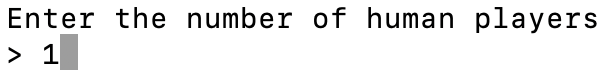
\includegraphics[width=8cm]{./images/human-players-village-war-game.png}
    \caption{Picking the number of human players}
    \label{human-players-village-war-game}
\end{figure}

\subsubsection*{\ul{Number of AI Players}}

\begin{figure}[H]
    \centering
    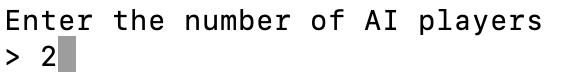
\includegraphics[width=8cm]{./images/ai-players-village-war-game.png}
    \caption{Picking the number of AI players}
    \label{ai-players-village-war-game}
\end{figure}

\begin{figure}[H]
    \centering
    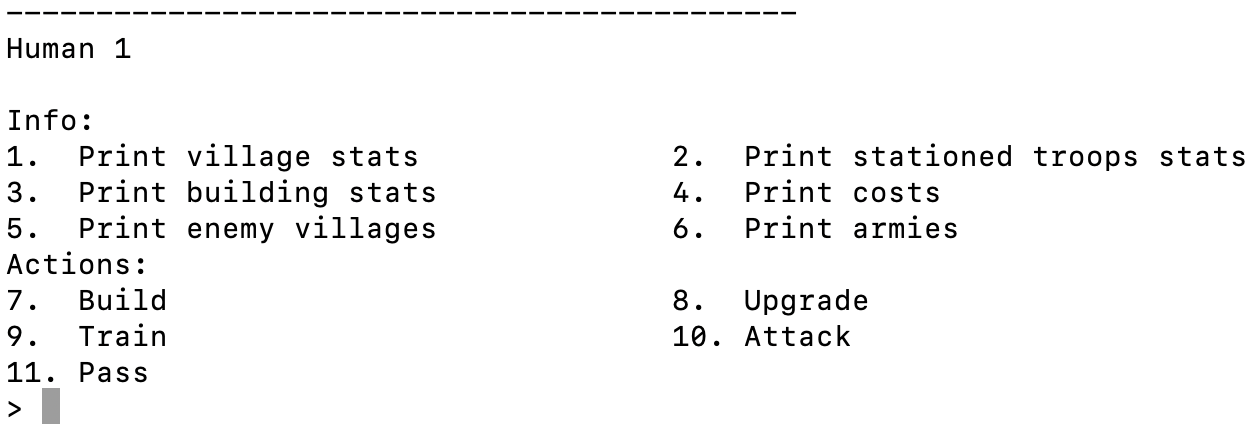
\includegraphics[width=12cm]{./images/player-menu-village-war-game.png}
    \caption{The menu for human players}
    \label{player-menu-village-war-game}
\end{figure}

Each human player is prompted with a menu of options having two
categories: \textbf{Info} and \textbf{Actions}.

The \textbf{Info} category contains options which provide the
player with information about his own village, enemy villages,
armies and costs. Every option is self--explanatory.

The \textbf{Actions} category contains options which affect the
state of the game, such as \textit{building}, \textit{upgrading}
\textit{training} and \textit{attacking}. A player can also
\textit{pass} the turn to the next player.

All players, by default, start with $50$ ``food'', ``metal'' and
``mana''. The player can use resources or troops to perform the
above described actions.

There are three types of troops:

\begin{enumerate}
    \item Wizard (high attack, low health, medium speed, low
        carrying capacity)
    \item Brawler (high attack, high health, slow speed, medium
        carrying capacity)
    \item Scout (medium attack, medium health, high speed, high
        carrying capacity)
\end{enumerate}

And there six types of building:

\begin{enumerate}
    \item Academy (to generate wizards)
    \item Foundation (to generate scouts)
    \item Arena (to generate brawlers)
    \item Farm (to generate food)
    \item Mine (to generate metal)
    \item Mana Tower (to generate mana)
\end{enumerate}

\textbf{Note:} It is useful to check the amount of resources you
have using option $1$ prior to performing any action.

\subsubsection*{\ul{Building}}

\begin{enumerate}
    \item Use option $7$ to get a list of all the different
        buildings and there build cost.
    \item Pick from option $1$ -- $6$ to build or $7$ to go
        back.
    \item You can view your new building by using option $3$.
\end{enumerate}

\subsubsection*{\ul{Upgrading}}

\begin{enumerate}
    \item Use option $8$ to get a list of all the different
        buildings and there upgrade cost.
    \item Pick from option $1$ -- $6$ to upgrade or $7$ to go
        back.
    \item You can view your upgraded building by using option $3$.
\end{enumerate}

\textbf{Note:} The player does not have granular control over
which buildings to upgrade. Given the implementation, the oldest
building of the specified type is upgraded first. However,
buildings which have reached their maximum level cannot be
upgraded further.

\subsubsection*{\ul{Training}}

\begin{enumerate}
    \item Use option $9$ to get a list of all the different
        troops and there training cost.
    \item Pick from option $1$ -- $3$ to train or $4$ to go
        back.
    \item Pick the number of troops to train.
    \item You can view the contribution of your trained troops
        by using option $2$.
\end{enumerate}

\textbf{Note:} The user does not have granular control over
which troops to train. Due to the movement of troops, they
are essentially trained randomly. However, troops which have
reached their maximum level cannot be trained further.

\subsubsection*{\ul{Attacking}}

\begin{enumerate}
    \item Use option $10$ to get a list of all enemy villages.
    \item Pick a village, from $1$ -- $n$, to attack.
    \item Pick the composition of the army i.e. the number of
        wizards, brawlers and scouts.
    \item You can view the marching armies by using option $6$.
\end{enumerate}

\subsubsection*{\ul{Quitting}}

Any human player can quit by pressing \texttt{Ctrl--C}.

\subsubsection*{\ul{Player Notification}}

In all instances where the player input is unexpected or
incorrect, the player is notified. All notification messages are
handled in the \texttt{HumanPlayer} class or using the
\texttt{Status} enum.

The most common notifications are caused by not having enough
troops or not having enough resources.

\subsection{Design}

\begin{figure}[H]
    \centering
    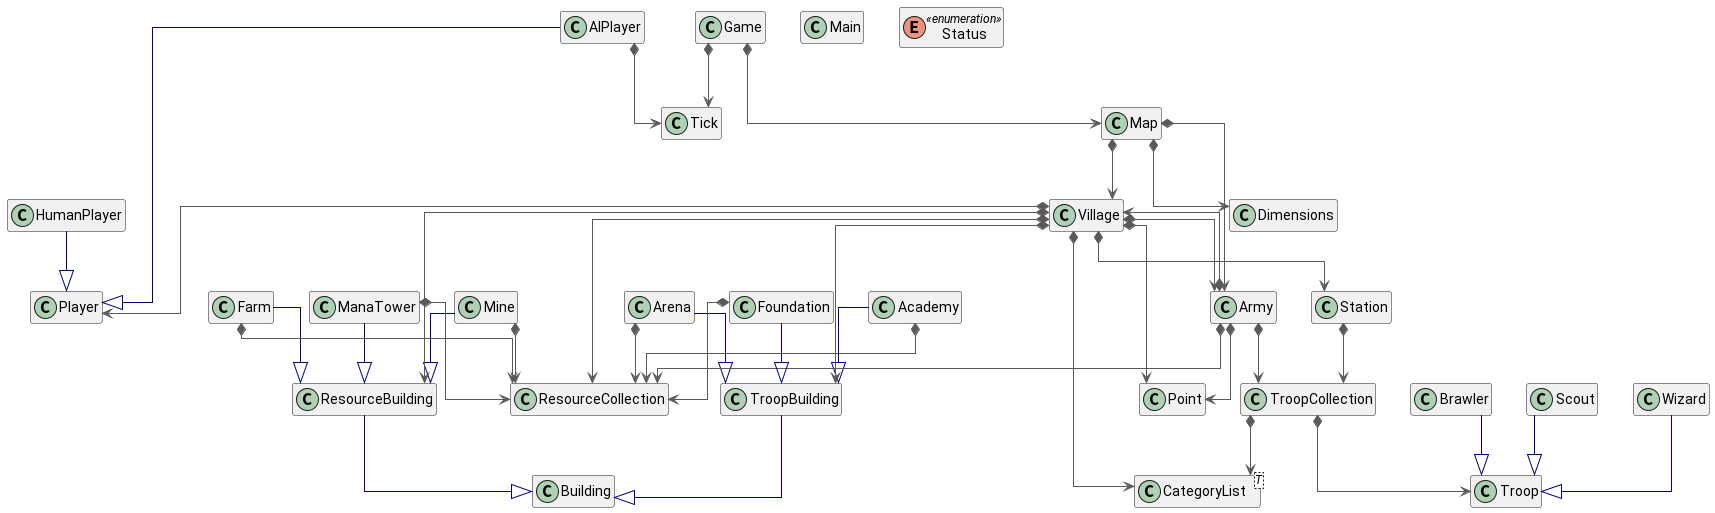
\includegraphics[width=17cm]{./village-war-game-uml/village-war-game.png}
    \caption{A UML diagram (without members) of the game}
\end{figure}

\textbf{Note:} The full UML diagram including members is not
shown as it would take up too much space.

\subsubsection{The Game Class}

The \texttt{Game} class is the entry point of the game. It
houses a \texttt{Map} object and has two main phases. The
\textit{setup} phase and the \textit{game--loop} phase.

The \textit{setup} phase creates and initialises all the objects
required at the start.

The \textit{game--loop} phase is where all the game play takes
place. Each iteration of the loop is called a ``round''. The
total number of rounds is tracked using a singleton
\texttt{Tick} object.

\textbf{Note:} The size of the map varies depending on the
number of players and the villages are spread out evenly across
the map.

\subsubsection{Map \& Village Design}

The \texttt{Map} class contains two lists: a list of villages
and a list of armies, and each village and army contains a
\texttt{Point} object to store its own location. This approach,
instead of using a 2D array has the benefit of allowing multiple
entities to exist at the same location. This is important since
marching armies can have intersecting paths. Moreover, it makes
managing entities significantly easier.

The village of each player is the hub where all actions are
performed. Unfortunately this means that the village has to be
polluted with a lot of action methods.

\subsubsection{Player Design}

For the player, there is a main abstract class and two
subclasses which implement the interface defined in the abstract
class. The two subclasses are \texttt{AIPlayer} and
\texttt{HumanPlayer}. Each village has a player and both types
of players interact with the village using the same methods
exposed by the \texttt{Village} class. This is because both
players have an \texttt{actions()} method which takes in a
\texttt{Village} object.

\textbf{Note:} A reference to the singleton \texttt{Tick} object
is present in all AI players. This allows for more complicated
AI behaviour because a whole game can be segmented into
different stages for example: the opening, the mid-game and the
end-game.

\subsubsection{Resource Design}

Since the resources carry no internal state and only the
quantity of the resources matters there is no need for creating
actual objects to represent the resources. Hence, everything was
designed around having a \texttt{ResourceCollection} class which
holds counters for each type of resource.

\subsubsection{Troop Design}

Again there is a \texttt{Troop} abstract class which specifies
the behaviour of all troops and then there are subclasses which
initialize their fields with specific values according to the
strengths and weaknesses each Troop type (as described above in
the player guide.)

Further more an important data structure built on top of the
\texttt{CategoryList} is the \texttt{TroopCollection}. This
class facilitates the grouping of all troops even of different
class types into one object. This object is able to send and
receive troops, calculate the total attack power etc.

Additionally, \texttt{Army} and \texttt{Station} are two other
classes which compose a \texttt{TroopCollection}. Armies are
different from stations because they are capable of marching
across the map and engaging in combat with an enemy village.
This is reflected in the additional methods and required fields.

\subsubsection{Building Design}

There is a main abstract class called \texttt{Building} and two
abstract subclasses called \texttt{TroopBuilding} and
\texttt{ResourceBuilding}. These two subclasses facilitate the
differentiation of troop--generating buildings and
resource--generating buildings. This split was done under the
assumption that the troop buildings require an additional method
to train troops. This was no longer the case later in
development. Removing two subclasses would have required quite a
few changes to the code. Consequently, the subclasses were kept.

Since training is not actually done by the building but by a
method in the \texttt{Troop} class, to follow the game
specification, a check was added to ensure that at least one
building of the appropriate type exists. 

\subsection{Technical Aspects}

\subsubsection{Usage of Exceptions}

Exceptions were avoided as they obscure control flow. Most
errors do not arise because of exceptional circumstances.
Exceptions were handled only when thrown from the standard
library.

\subsubsection{OOP \& \texttt{CategoryList}}

Using OOP and creating separate classes for the building and
troop types added complexity to the code. This is because when
it comes to generics and reflection Java is quite limited. This
became an issue, because when trying to genericise the code to
cater for multiple troop and building types, without needing to
change the \texttt{Village} class, it proved to be very difficult.

It required the creation of a special data structure named a
\texttt{CategoryList}. It is similar to a \texttt{HashMap},
however, the key is the type of the object. This data structure
facilitates: getting a collection of objects by there type,
iterating over all objects etc. However, it is still limited
because it is not capable of handling multi--level inheritance
hierarchies.

\subsubsection{Singleton Design Pattern}

Some objects such as \texttt{Tick} and \texttt{Map} require only
one instance for the whole game. Hence, the singleton pattern
was used for these objects.

\subsubsection{Observer Design Pattern}

When an army is defeated, following the specification, the army
is also destroyed. This requires that the player is notified
about the defeat as it is information which can affect the
decisions the player takes. Hence, the observer pattern is used
to notify the player about the armies defeat.

To handle this properly a message queue was added to the
\texttt{HumanPlayer} class to keep track of all the
notifications. Then at every turn all received notifications
will be printed. This ensures that notifications do not clutter
the UI.

\subsection{Testing}

There are three types of failures which our application has
to cater for:

\begin{enumerate}
    \item Failure due to the inability to parse player input.
    \item Failure due to invalid or out--of--bounds input.
    \item Failure due to insufficient resources or troops.
\end{enumerate}

\begin{figure}[H]
    \centering
    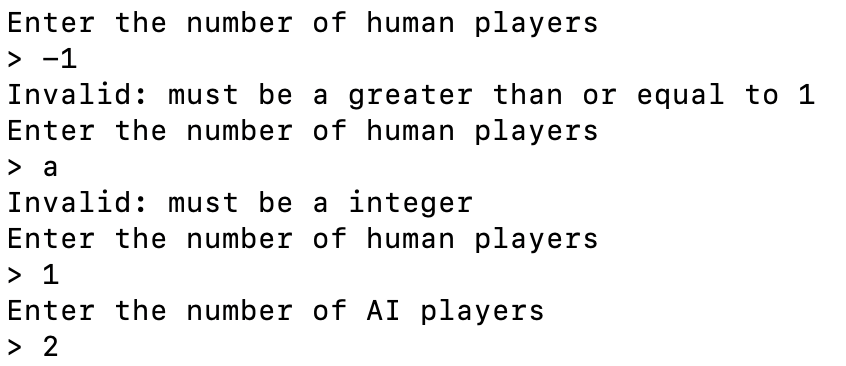
\includegraphics[width=10cm]{./images/invalid-user-input-village-war-game.png}
    \caption{Demonstrating failure due to invalid option
    (out--of--bounds) and the inability to parse respectively}
\end{figure}

\begin{figure}[H]
    \centering
    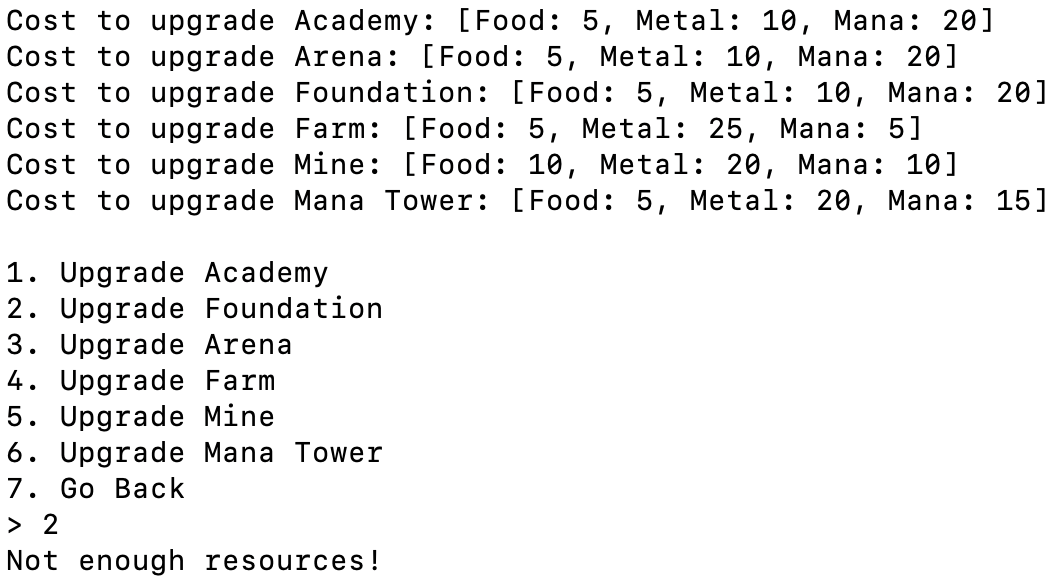
\includegraphics[width=10cm]{./images/not-enough-resources-village-war-game.png}
    \caption{Demonstrating failure due to insufficient
    resources}
\end{figure}

Each input was manually tested to ensure that the above three
cases are handled properly.

\begin{figure}[H]
    \centering
    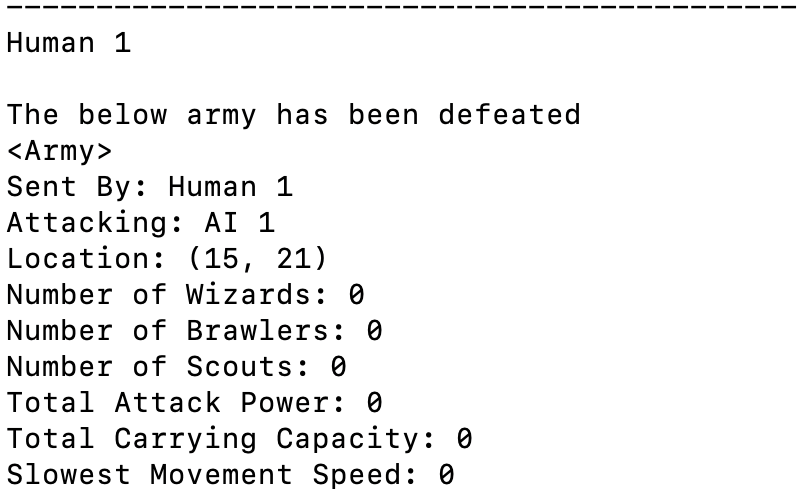
\includegraphics[width=10cm]{./images/testing-army-defeat-village-war-game.png}
    \caption{Demonstration of a army defeat notification}
\end{figure}

Additionally, the game was further manually tested in a form of
white-box testing to ensure that behaviour is as expected.

\subsection{Limitations \& Improvements}

\ul{Limitation:} The user interface is very limiting. It is
limited in the amount of information it can neatly provide to
the player, it is limited in maneuverability etc.

\ul{Solution:} Using a GUI would help provide a better UX since
a GUI is very flexible.

\ul{Limitation:} The amount of control the player has, is
limited. This is mainly due to how clunky the UI is. Giving the
user more granular control would require more clutter or more
nesting in sub--menus. 

\ul{Solution:} Changing to GUI can allow the application to grow
in terms of complexity without sacrificing UX.

\section{Minesweeper}

\subsection{Language Choice}

\cpp{} was chosen for Minesweeper because it has a fixed board
size of $16 \times 16$. This means that it is possible to stack
allocate every object removing the need for dynamic memory
allocation. This is facilitated by \texttt{std::array} from the
Standard Template Library (STL) which allows for the creation of
fixed size arrays on the stack.

\subsection{User Guide}

\subsubsection{Download, Compiling \& Running}

\begin{enumerate}
\item
    Clone the repository.
\begin{lstlisting}
$ git clone https://github.com/JuanScerriE/minesweeper
\end{lstlisting}

\item
    Compile the tests and the game.

    \textbf{Note:} Make sure that \texttt{gtest} and
    \texttt{ncurses} are installed for the tests and the game,
    respectively.
\begin{lstlisting}
$ cd minesweeper ; ./compile.sh
\end{lstlisting}

\item
    Run the tests.

    \textbf{Note:} Some tests might fail. This is because the
    implementation of \texttt{srand} and \texttt{rand} differ
    between platforms (specifically macOS and Linux).
\begin{lstlisting}
minesweeper $ ./tests.sh
\end{lstlisting}

\item
    Run the game.
\begin{lstlisting}
minesweeper $ ./run.sh
\end{lstlisting}

\end{enumerate}

\subsubsection{Playing}

\begin{figure}[H]
    \centering
    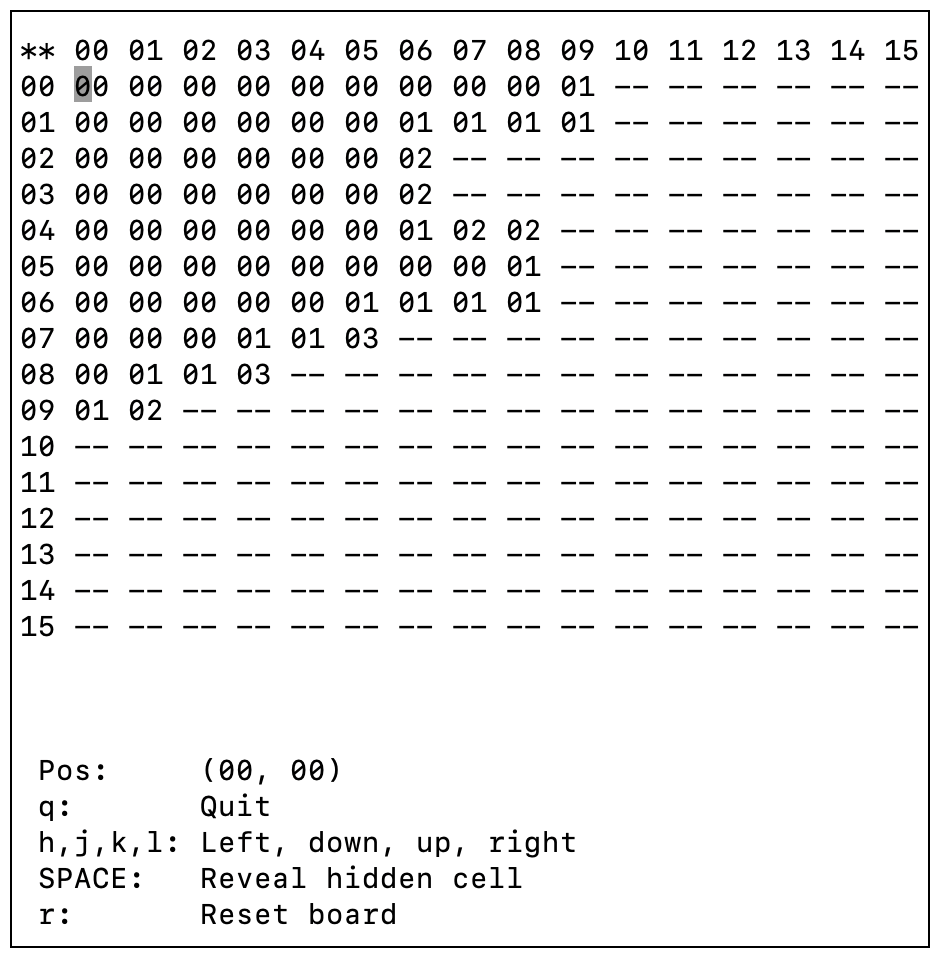
\includegraphics[width=8cm]{./images/playing-minesweeper.png}
    \caption{Playing Minesweeper}
    \label{playing-minesweeper}
\end{figure}

The general guide to playing Minesweeper is described above in
figure \ref{playing-minesweeper}.

\textbf{Note:} \texttt{vim} motions are used to move the cursor.

If the player hits a mine the message ``YOU HAVE HIT A MINE!
(Press r to retry)'' will be displayed. 

If the player manages to clear all the cells without hitting a
mine the message ``YOU HAVE CLEARED THE BOARD! (Press r to
retry)'' will be displayed.

Finally, there is an additional \textit{secret} command to
automatically complete the board without hitting a mine. The
user needs to press \texttt{W} (\texttt{Shift--W}).

\textbf{Note:} This only works if the user has at least revealed
one cell. This is because the board is populated with all the
mines after the first reveal to ensure a player never hits a
mine on his first try.

\subsection{Design}

\begin{figure}[H]
    \centering
    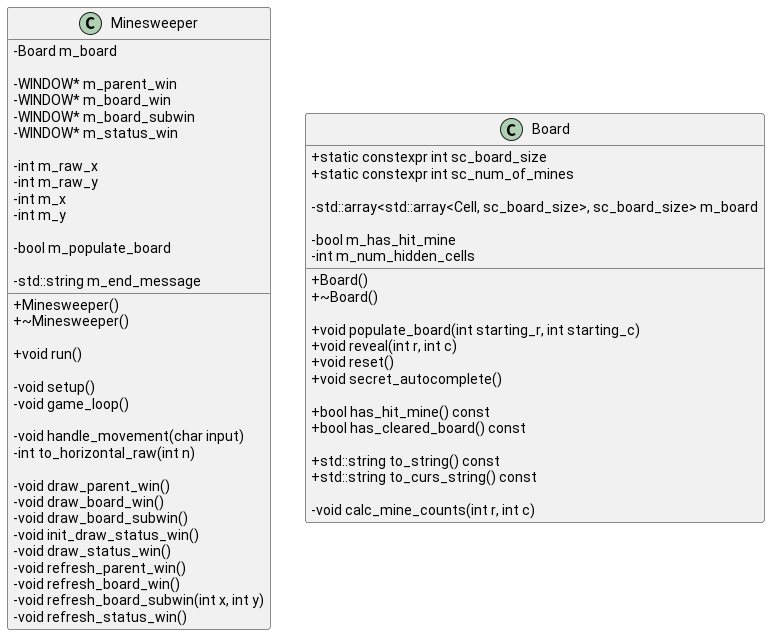
\includegraphics[width=12cm]{minesweeper-uml/minesweeper-and-board.png}
    \caption{Class diagrams of the Minesweeper class and the Board class}
\end{figure}

The Minesweeper class contains the user interface code, that
is it contains all \texttt{ncurses} specific code. The class
also handles user input.

The Board class contains the majority of the game logic. It is a
part of the Minesweeper class, that is if a Minesweeper object
ceases to exist so does the Board object.

\begin{figure}[H]
    \centering
    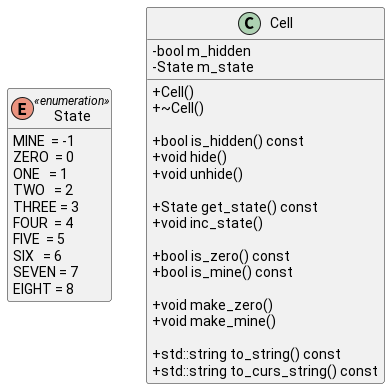
\includegraphics[height=8cm]{minesweeper-uml/cell.png}
    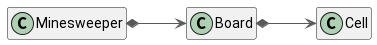
\includegraphics[width=12cm]{minesweeper-uml/relations.png}
    \caption{A class diagram of the Cell class State enum and a
    UML diagram (without members) of the game}
\end{figure}

Furthermore, the actual board \texttt{m\_board} is a grid of
Cell objects. Also, the lifetime of the objects is managed by
the Board as when the board ceases to exist so do the cells.

\subsection{Testing}

\begin{figure}[H]
    \centering
    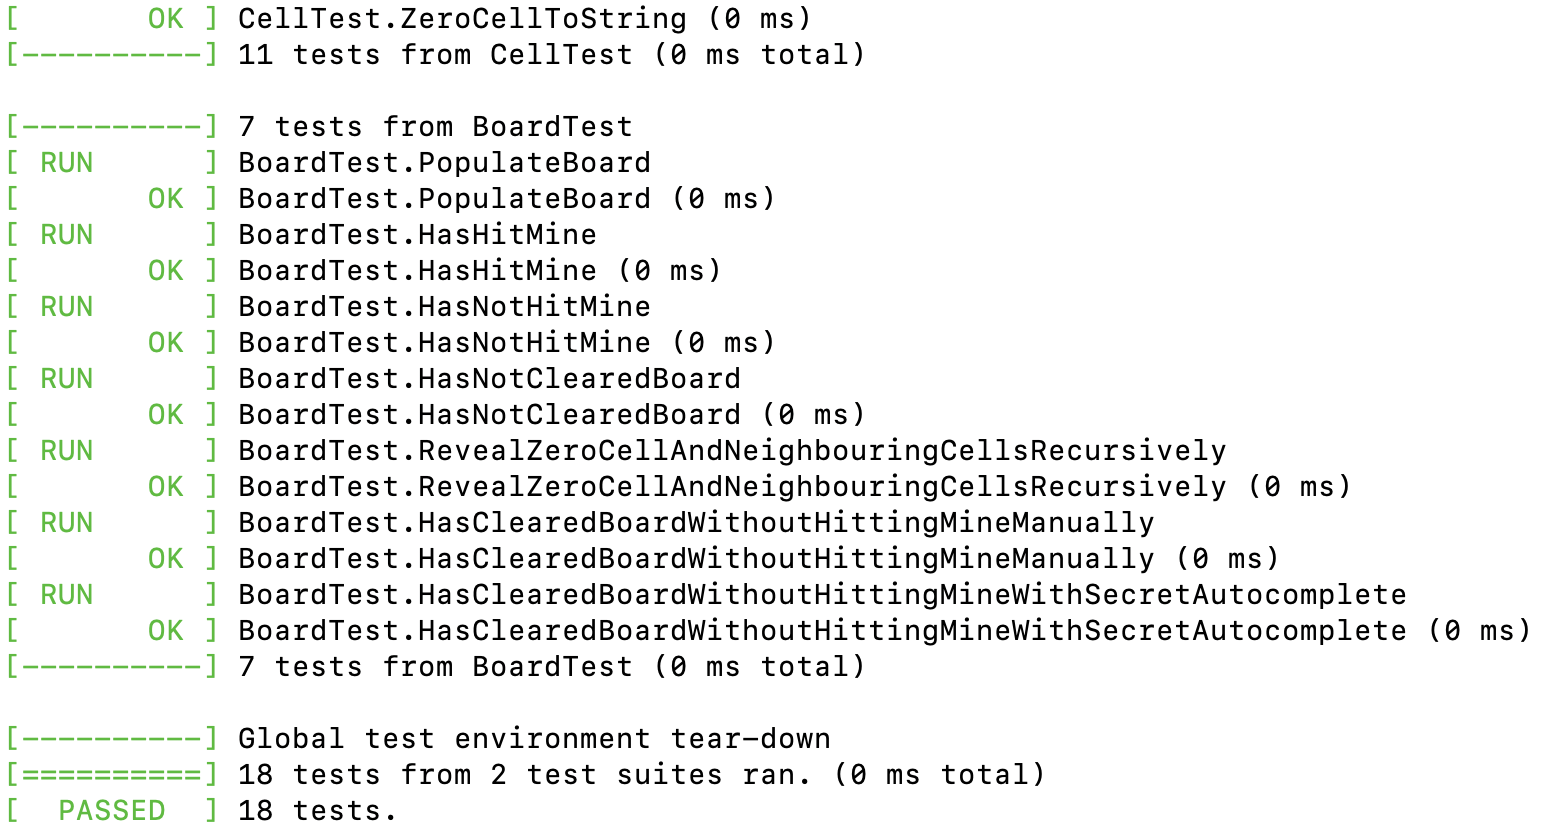
\includegraphics[width=8cm]{./images/unit-tests-minesweeper.png}
    \caption{Unit tests for Minesweeper (on macOS Ventura 13.1)}
\end{figure}

White--box Testing and Unit Testing were used to test the
application. For unit testing \texttt{gtest} is required.

\begin{figure}[H]
    \centering
    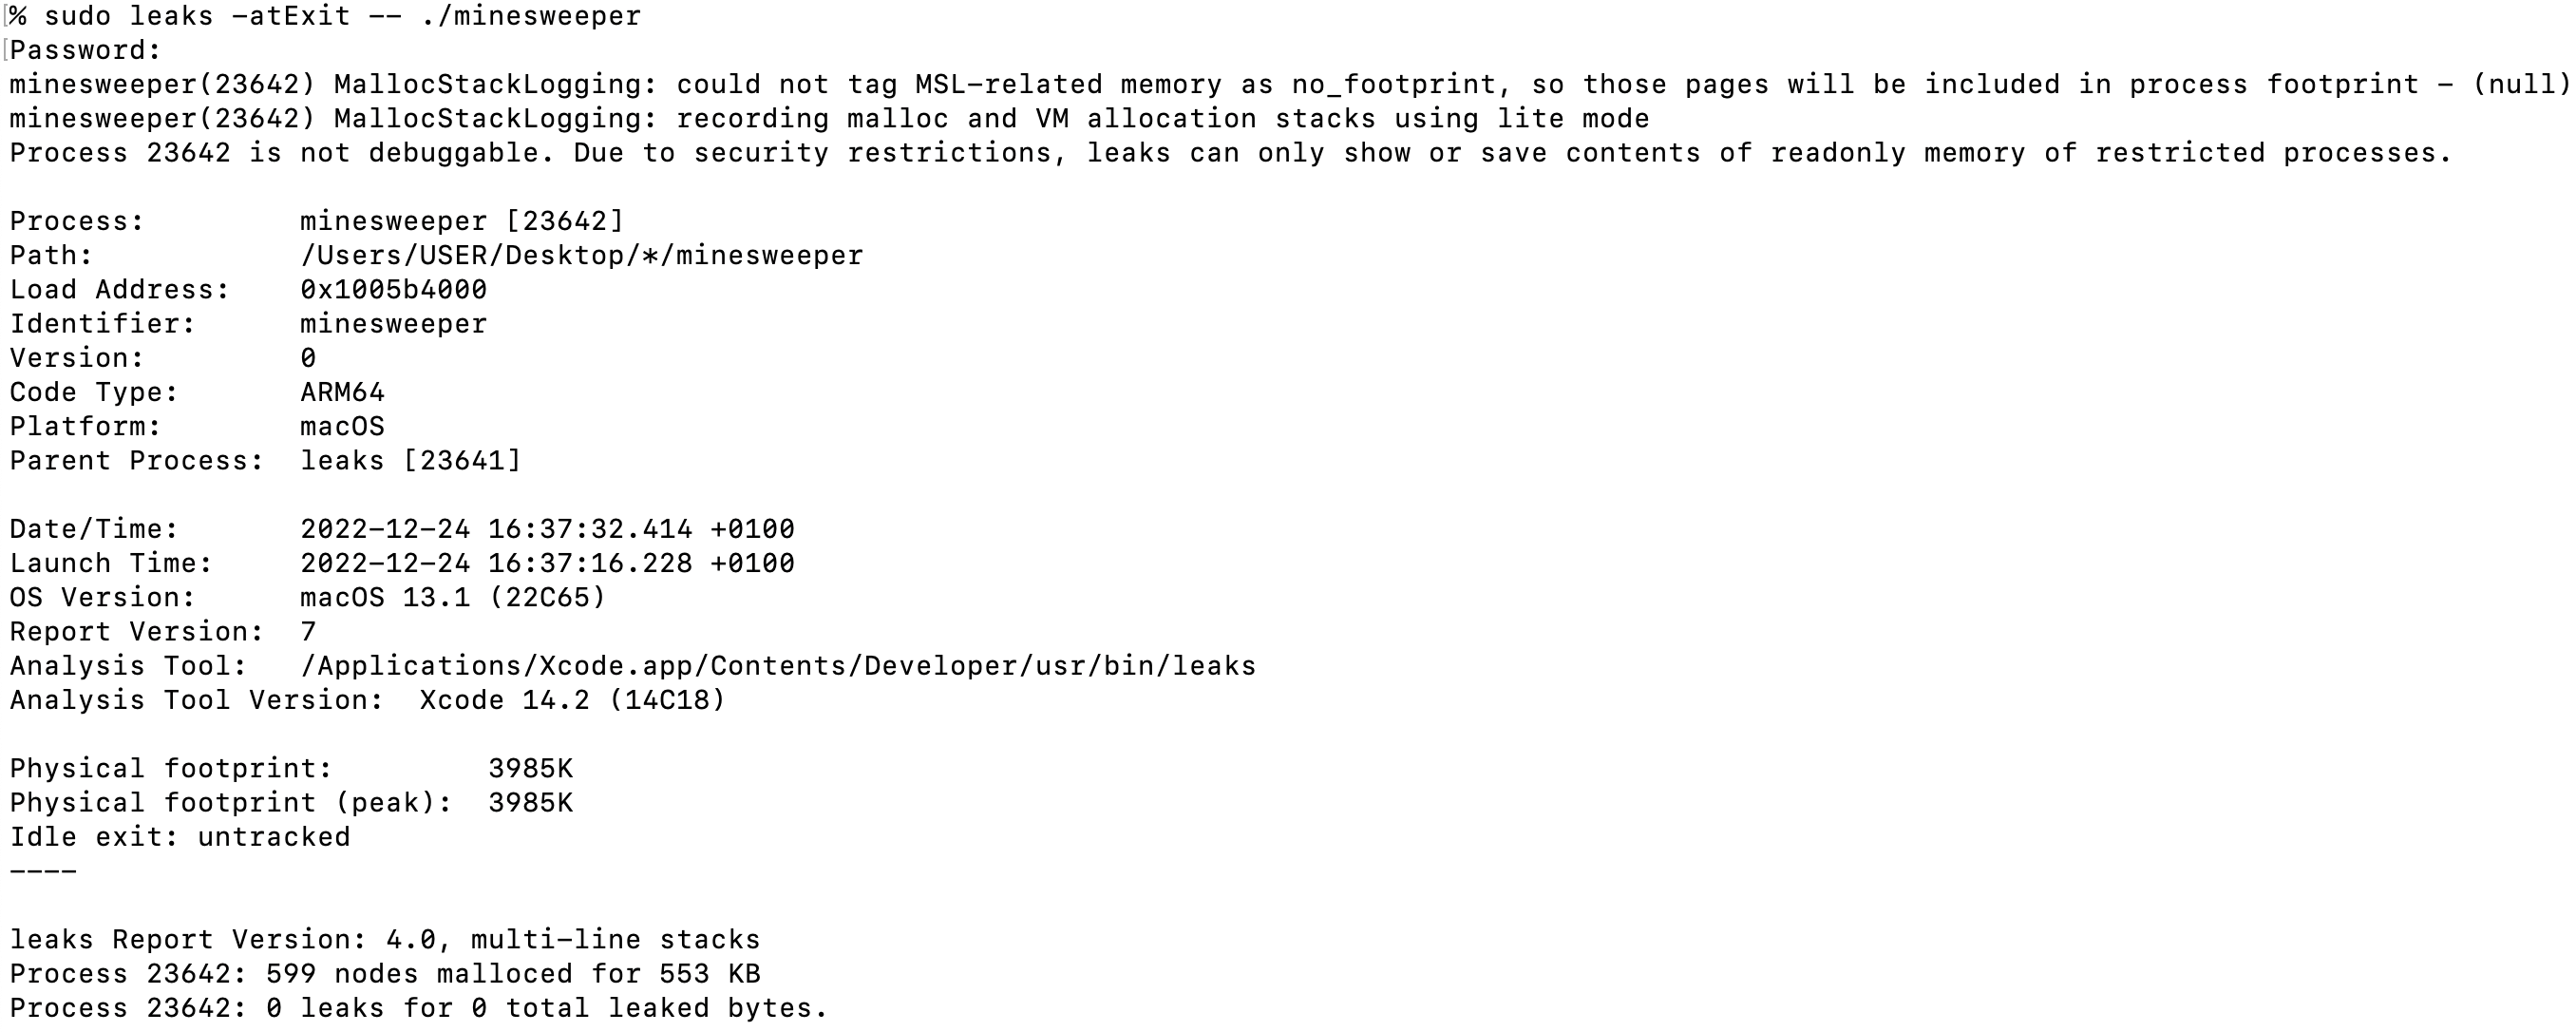
\includegraphics[width=14cm]{./images/leaks-minesweeper.png}
    \caption{Testing for memory leaks (on macOS Ventura 13.1)}
\end{figure}

Furthermore, to test for memory leaks, \texttt{leaks} was used
on macOS and \texttt{valgrind} was used on Linux. \texttt{leaks}
reported no memory leaks whilst \texttt{valgrind} reported
leaks from \texttt{ncurses}.

\subsection{Limitations \& Improvements}

\ul{Limitation:} The unit tests are not cross-platform; four of
the unit tests fail on Linux. This is mostly due to differing
implementations of \texttt{srand()} and \texttt{rand()} on
different platforms.

\ul{Solution:} Create a custom random number generated. This
guarantees the same result across different platforms.

\ul{Limitation:} The \texttt{ncurses} library leaks memory on
Linux whilst it does not on macOS.

\ul{Solution:} This seems to be intended behaviour from
\texttt{ncurses}. Read the man page at
\url{https://man7.org/linux/man-pages/man3/curs_memleaks.3x.html}

\end{document}
